
\documentclass[11pt]{article} % use larger type; default would be 10pt

%%% ----------------------------------------------------------
%%% Addings
\input{../latex_additions/__technical_additions}
%%% End of the addings
%%% ----------------------------------------------------------




\title{Algorithmique\\ -- version 0.1}
\date{\vspace{-5ex}}
\author{Dr M. GUEDJ}

\begin{document}



\renewcommand{\contentsname}{Table des Matières}
\maketitle


%%%%%%%%%%%%%%%%%%%%%%%%%%%%%% LICENCE CC %%%%%%%%%%%%%%%%%%%%%%%%%%%%
\newpage
\begin{center}
\includegraphics[scale=0.5]{licence/licence_cc.png}

\begin{small}
Algorithmique de Dr Michaël GUEDJ est mis à disposition selon les termes de la licence Creative Commons Attribution 4.0 International.
Fondé(e) sur une œuvre à 
\url{https://github.com/michaelguedj/ens__algorithmique}.
\end{small}
\end{center}
\newpage
%%%%%%%%%%%%%%%%%%%%%%%%%%%%%%%%%%%%%%%%%%%%%%%%%%%%%%%%%%%%%%%%%%%%%%


\tableofcontents
%%%
%%%

\newpage
\section{Algorithmes sur tableaux}



%%%
\subsection{Un tableau est-il vide ?}
\begin{algorithm}[H]
\caption{$\algo{est\_vide}$ ($t$ : tableau, $n$ : taille du tableau)}
\begin{algorithmic}[1]
\If{$n=0$}
	\State\Return $\True$
\Else
	\State\Return $\False$
\EndIf
\end{algorithmic}
\end{algorithm}

Complexité : $O(1)$.


%%%
\subsection{Afficher les éléments d'un tableau}
\begin{algorithm}[H]
\caption{\algo{afficher\_tableau} ($t$ : tableau, $n$ : taille du tableau)}
\begin{algorithmic}[1]
\For{$i \gets 0, ..., n-1$}
	\State \print($t[i]$)
\EndFor
\end{algorithmic}
\end{algorithm}

Complexité : $O(n)$.


%%%
\subsection{Afficher les éléments positifs d'un tableau}
\begin{algorithm}[H]
\caption{\algo{afficher\_positifs} ($t$ : tableau, $n$ : taille du tableau)}
\begin{algorithmic}[1]
\For{$i \gets 0, ..., n-1$}
	\If{$t[i]\geq 0$}
		\State \print($t[i]$)
	\EndIf
\EndFor
\end{algorithmic}
\end{algorithm}

Complexité : $O(n)$.


%%%
\subsection{Retourner l'éléments maximum d'un tableau}
\begin{algorithm}[H]
\caption{\algo{maximum} ($t$ : tableau, $n$ : taille du tableau)}
\begin{algorithmic}[1]
\State \green{\Comment{On suppose $n>0$}}
\State $max \gets t[0]$ 
\For{$i \gets 1, ..., n-1$}
	\If{$t[i]\geq max$}
		\State $max \gets t[i]$
	\EndIf
\EndFor
\State\Return $max$
\end{algorithmic}
\end{algorithm}


Complexité : $O(n)$.


%%%
\subsection{Retourner l'indice de l'éléments maximum d'un tableau}
\begin{algorithm}[H]
\caption{\algo{inidice\_maximum} ($t$ : tableau, $n$ : taille du tableau)}
\begin{algorithmic}[1]
\State \green{\Comment{On suppose $n>0$}}
\State $max \gets t[0]$ 
\State $iMax \gets 0$ 
\For{$i \gets 1, ..., n-1$}
	\If{$t[i]\geq max$}
		\State $max \gets t[i]$
		\State $iMax \gets i$
	\EndIf
\EndFor
\State\Return $iMax$
\end{algorithmic}
\end{algorithm}

Complexité : $O(n)$.


%%%
\subsection{Retourner la somme des éléments d'un tableau}
\begin{algorithm}[H]
\caption{\algo{somme} ($t$ : tableau, $n$ : taille du tableau)}
\begin{algorithmic}[1]
\State $res \gets 0$ 
\For{$i \gets 0, ..., n-1$}
	\State $res \gets res + t[i]$
\EndFor
\State\Return $res$
\end{algorithmic}
\end{algorithm}

Complexité : $O(n)$.


%%%
\subsection{Rechercher un élément dans un tableau}
\begin{algorithm}[H]
\caption{\algo{recherche} ($t$ : tableau, $n$ : taille du tableau, $x$ : élément)}
\begin{algorithmic}[1]
\For{$i \gets 0, ..., n-1$}
	\If{$t[i] = x$}
		\State\Return $\True$
	\EndIf
\EndFor
\State\Return $\False$
\end{algorithmic}
\end{algorithm}

Complexité : $O(n)$.


%\newpage
%\section{Liste cha\^inée, pile et file }
%


\subsection{Liste cha\^inée}

\begin{itemize}
\item[--] \textbf{est\_vide} : retourne $\True$ si la liste est vide ; et $\False$ sinon ;
\item[--] \textbf{taille} : retourne le nombre d'éléments dans la liste ;
\item[--] \textbf{insérer\_après} : insére un élément après l'élément passé en argument ;
\item[--] \textbf{insérer\_en\_tête} : insére un élément avant le premier élément de la liste ;
\item[--] \textbf{supprimer\_après} : insére un élément après l'élément passé en argument ;
\item[--] \textbf{supprimer\_en\_tête} : supprime le premier élément de la liste.
\end{itemize}



\subsection{Pile}

\begin{itemize}
\item[--] \textbf{est\_vide} : retourne $\True$ si la pile est vide et $\False$ sinon ;
\item[--] \textbf{taille} : renvoie le nombre d'éléments dans la pile ;
\item[--] \textbf{empiler} : ajoute un élément sur la pile ;
\item[--] \textbf{dépiler} : enlève un élément de la pile et le retourne ;
\item[--] \textbf{sommet} : retourne l'élément de tête sans le dépiler.
\end{itemize}



\subsection{File}
\begin{itemize}
\item[--] \textbf{est\_vide} : retourne $\True$ si la file est vide, et $\False$ sinon ;
\item[--] \textbf{taille} : retourne le nombre d'éléments dans la file ;
\item[--] \textbf{enfiler} : ajoute un élément dans la file ;
\item[--] \textbf{défiler} : retourne le prochain élément de la file, et le retire de la file.
\end{itemize}


\newpage
\section{Algorithmes sur matrices}



%%%
%%%
\subsection{Afficher les éléments d'une matrice}
\begin{algorithm}[H]
\caption{\algo{afficher\_matrice} ($A$ : matrice $n\times m$)}
\begin{algorithmic}[1]
\For{$i \gets 0, ..., n-1$}	\green{\Comment{parcours sur les lignes}}
	\For{$j \gets 0, ..., m-1$}	\green{\Comment{parcours sur les colonnes}}
		\State \print($A_{i,j}$)
	\EndFor
	\State \print(saut de ligne)
\EndFor
\end{algorithmic}
\end{algorithm}

Complexité : $O(n\times m)$.

\noindent
Cas d'une matrice carré $n\times n$ : $O(n^2)$ (complexité linéaire !).

%%%
%%%
%%%
%%%
%%%
%%%
\subsection{Additionner deux matrices}
\begin{algorithm}[H]
\caption{\algo{additionner} ($A, B$ : matrice $n\times m$)}
\begin{algorithmic}[1]
\State $C \gets$ matrice $n\times m$
\For{$i \gets 0, ..., n-1$}
	\For{$j \gets 0, ..., m-1$}
		\State $C_{i, j}\gets A_{i,j} + B_{i,j}$
	\EndFor
\EndFor
\State\Return $C$
\end{algorithmic}
\end{algorithm}

Complexité : $O(n\times m)$.


%%%
%%%
%%%
%%%
%%%
%%%
\subsection{La matrice est-telle diagonale ?}

Rappel : la matrice carré $n\times n$, soit $M$, est diagonale si :
$$\forall i,j\in\{0, ..., n-1\}, 
i\not=j \Rightarrow M_{i,j}=0$$

\begin{algorithm}[H]
\caption{\algo{est\_diagonale} ($M$ : matrice $n\times n$)}
\begin{algorithmic}[1]
\For{$i \gets 0, ..., n-1$}
	\For{$j \gets 0, ..., n-1$}
		\If{$i\not=j$ et $M_{i,j}\not=0$}
			\State\Return $\False$
		\EndIf
	\EndFor
\EndFor
\State\Return $\True$
\end{algorithmic}
\end{algorithm}

Complexité : $O(n^2)$.



\newpage
\section{Complexité en temps (cas le pire)}


\subsection{Approximation asymptotique}
\blue{
\begin{fDefinition}[Notation grand O]
Soient $f$ et $g$ deux fonctions de $\mathbb{N} \rightarrow \mathbb{R}^{+}$.
$f \in O(g)$ si :
\begin{itemize}
\item[--] $\exists K \in\mathbb{R}^{*+}$ ;
\item[--] $\exists n_0 \in \mathbb{N}$ ; 
\end{itemize}
et
$$
\forall n\geq n_0,~ f(n) \leq K. g(n)
$$
($f(n) \leq K. g(n)$ à partir d'un certain rang). 
\end{fDefinition}
}

%\noindent
\textbf{Exemples}
\begin{itemize}
\item[--] $7n-3 \in O(n)$
\item[--] $7n-3 \in O(n^2)$
\item[--] $987654321 + 10n^2 \in O(n^2)$
\end{itemize}

\noindent
\textbf{Remarque}
Le but est de trouver l'approximation la plus petite possible.


%%%%
%%%%
%%%%
%%%%
%%%%
\subsection{Complexités en temps classiques}
\begin{tabular}{|l|l|l|}
  \hline
  \textbf{Complexité} & \textbf{Notation asymptotique} & \textbf{Exemple} \\
  \hline
  Logarithmique 	& $O(\log n)$			& Recherche dichotomique dans un tableau trié. \\
  \hline
  Linéaire 		& $O(n)$ 				& Recherche séquentielle dans un tableau. \\
  \hline
  Quasi-linéaire  & $O(n \log n)$ 		& Tri fusion. \\
  \hline
  Quadratique 	& $O(n^2)$ 			& Tri sélection; tri à bulles.\\
  \hline
  Polynomiale 	& $O(n^k), k\geq 0$	& $~$... \\
  \hline
  Exponentielle 	& $O(k^n), k>1$ 		& Algorithme récursif pour Fibonacci. \\
  \hline
  Factorielle 	& $O(n!)$ 			& Résolution des $n$-reines par \textit{backtracking}. \\
  \hline
\end{tabular}

%%%%
%%%%
%\subsection{Comparaisons}
%$$
%\log n \ll n \ll n \log n \ll n^2 \ll n^3 \ll 2^n \ll n!
%$$


\newpage
\section{Tris quadratiques }


\subsection{Algorithme d'échange}

\begin{algorithm}[H]
\caption{\algo{echanger}($t$ : tableau, $i,j$ : entiers)}
\begin{algorithmic}[1]
\State $tmp \gets t[i]$ 
\State $t[i] \gets t[j]$ 
\State $t[j] \gets tmp$ 
\end{algorithmic}
\end{algorithm}



\subsection{Tri par sélection}

\begin{algorithm}[H]
\caption{\algo{tri\_selection}($t$ : tableau, $n$ : taille du tableau)}
\begin{algorithmic}[1]
\For{$i\gets 0, ..., n-2$}
	\State $i_{min} \gets $ $\algo{indice\_min\_sous\_tab}(t, i, n-1)$
	\State $\algo{echanger}(t, i, i_{min})$ 
\EndFor
\end{algorithmic}
\end{algorithm}

\begin{algorithm}[H]
\caption{\algo{indice\_min\_sous\_tab}($t$ : tableau, $a, b$ : entiers)}
\label{indiceMin}
\begin{algorithmic}[1]
\State $i_{min} \gets a$
\For{$i\gets a+1, ..., b$}
	\If{$t[i] < t[i_{min}]$}
		\State $i_{min} \gets i$
	\EndIf
\EndFor
\State\Return $i_{min}$
\end{algorithmic}
\end{algorithm}

%%%%%%%%%%%%%%%%%%%%%%%%%%%%%%%%%%%%%%%%%%%%%%%%%%%%%
%%%%%%%%%%%%%%%%%%%%%%%%%%%%%%%%%%%%%%%%%%%%%%%%%%%%%
\blue{
\begin{fTheorem}
La complexité de $\algo{tri\_selection}$ est en $O(n^2)$.
\end{fTheorem}
}

\blue{
\begin{fTheorem}
Le nombre de comparaisons de $\algo{tri\_selection}$ est en $O(n^2)$.
\end{fTheorem}
}

\begin{proof}[Preuve]
Calcul du nombre de comparaisons $\mC(n)$ 
(ligne 3 de l'algorithme \ref{indiceMin}).
$$
\mC(n) = \sum_{i=0}^{n-2} \sum_{j=i+1}^{n-1} 1
$$
%
$$
\mC(n)
 = \sum_{i=0}^{n-2} 
								\Big(
										(n-1) - (i+1) + 1 
								\Big)
$$
%
$$
\mC(n)
 = \sum_{i=0}^{n-2} 
								\big(
										n-1 - i-1 + 1 
								\big)
$$
%
$$
\mC(n)
 = \sum_{i=0}^{n-2} 
								\big(
										n-1 - i 
								\big)
$$
%
$$
\mC(n) = 
 \sum_{i=0}^{n-2} (n-1)
-  \sum_{i=0}^{n-2} i
$$
%
$$
\mC(n) = 
 (n-1) \sum_{i=0}^{n-2} 1
-  \sum_{i=0}^{n-2} i
$$
%
$$
\mC(n) = 
	(n-1)(n-1)
	- \sum_{i=0}^{n-2} i 	
$$
%
$$
\mC(n) = 
	(n-1)^2
	- \sum_{i=0}^{n-2} i 	
$$
$$
\mC(n) = 
	(n-1)^2
	- \frac{(n-2)(n-1)} {2}
$$
%
$$
\mC(n) = 
	(n-1)
	\Big(
		(n-1)
		-\frac{(n-2) } {2}
	\Big)
$$
%
$$
\mC(n) = 
	(n-1)
	\Big(
		\frac{2.(n-1) -(n-2) } {2}
	\Big)
$$
%
$$
\mC(n) = 
	(n-1)
	\Big(
		\frac{2n-2 - n+ 2 } {2}
	\Big)
$$
%
$$
\mC(n) = 
	(n-1)
	\frac{n} {2}
$$
$$
\mC(n) = 
 	\frac{n^2}{2}
	-
	\frac{n}{2} \in O(n^2)
  	$$
\end{proof}


%%%%%%%%%%%%%%%%%%%%%%%%%%%%%%%%%%%%%%%%%%%%%%%%%%%%%%%%%%%%%%%%
%%%%%%%%%%%%%%%%%%%%%%%%%%%%%%%%%%%%%%%%%%%%%%%%%%%%%%%%%%%%%%%%
%%%%%%%%%%%%%%%%%%%%%%%%%%%%%%%%%%%%%%%%%%%%%%%%%%%%%%%%%%%%%%%%
\subsection{Tri à bulles}

\begin{algorithm}[H]
\caption{\algo{tri\_bulles}($t$ : tableau, $n$ : taille du tableau)}
\label{triBulles}
\begin{algorithmic}[1]
\For{$i \gets n-1, ..., 1$}
	\For{$j \gets 0, ..., i-1$}
		\If{$t[j+1] < t[j]$}
			\State $\algo{echanger}(t, j+1, j)$
		\EndIf
	\EndFor
\EndFor
\end{algorithmic}
\end{algorithm}


%%%%%%%%%%%%%%%%%%%%%%%%%%%%%%%%%%%%%%%%%%%%%%%%%%%%%
%%%%%%%%%%%%%%%%%%%%%%%%%%%%%%%%%%%%%%%%%%%%%%%%%%%%%
\blue{
\begin{fTheorem}
La complexité de $\algo{tri\_bulles}$ est en $O(n^2)$.
\end{fTheorem}
}

\blue{
\begin{fTheorem}
Le nombre de comparaisons de $\algo{tri\_bulles}$ est en $O(n^2)$.
\end{fTheorem}
}


\begin{proof}[Preuve]
Calcul du nombre de comparaisons $\mC(n)$ (ligne 4 de Algorithme \ref{triBulles}).
$$
\mC(n) = 
	\sum_{i=n-1}^{1} \sum_{j=0}^{i-1} 1 
 =
 	\sum_{i=n-1}^{1} (i-1-0+1) 
 = 
  	\sum_{i=n-1}^{1} i 
$$
%
$$
\mC(n) = 
   	\frac{(n-1+1) (n-1)}{2}
 =
    \frac{n (n-1)}{2}
 = \frac{n^2}{2} - \frac{n}{2} \in O(n^2)
  	$$
\end{proof}



\newpage
\section{Récursivité}





%%%
\subsection{Considérations sur la récursivité}

La version itérative d'un traitement est souvent à préférer.

En effet :
\begin{itemize}
	\item[--] Un dépassement de pile (\textit{stack overflow}) peut se produire ;
	\item[--] L'exécution d'une version récursive d'un algorithme est généralement un peu moins rapide 
			que celle de la version itérative correspondante ; 
			et ce même si le nombre d'instructions est le même (à cause de la gestion des appels de fonction) ;
	\item[--] Un algorithme récursif (naïf) peut conduire à exécuter bien plus d'instructions 
			que la version itérative correspondante (cas du calcul de la suite de Fibonacci).
\end{itemize}

\noindent
En revanche, la récursivité peut être adaptée dans certains cas.

En effet :
\begin{itemize}
	\item[--] Sur des structures de données naturellement récursives, 
	il est plus facile d'écrire des algorithmes récursifs qu'itératifs ;
	\item[--] Certains algorithmes sont, en outre, difficiles à écrire en itératif.
\end{itemize}


%%%
\subsection{Exemple 1 : la fonction factorielle}
\blue{
\begin{fDefinition}[fonction factorielle]
La fonction factorielle est définie, sur $\mathbb{N}$, par :
$$
\left\{
    \begin{array}{ll}
        0! = 1 						& \\
        n! = \Pi_{i=1}^{n} i = n\times (n-1) \times ... \times 2 \times 1 & \mbox{ si } n\geq 1
    \end{array}
\right.
$$
\end{fDefinition}
}

\blue{
\begin{fDefinition}[définition récursive de la fonction factorielle]
$$
n! = 
\left\{
    \begin{array}{ll}
        0 			& \mbox{si } n=0\\
        n\times (n-1)! & \mbox{si } n\geq 1
    \end{array}
\right.
$$
\end{fDefinition}
}

\begin{algorithm}[H]
\caption{$\algo{fact}(n\in\mathbb{N})$}
\begin{algorithmic}[1]
\If{$n = 0$}
	\State\Return 1
\Else
	\State\Return $n \times \textsc{fact}(n-1)$
\EndIf
\end{algorithmic}
\end{algorithm}

Complexité : $O(n)$


\begin{algorithm}[H]
\caption{$\algo{fact\_it}(n\in\mathbb{N})$}
\begin{algorithmic}[1]
\State $res\gets 1$
\For{$i\gets 1, ..., n$}
	\State $res \gets res \times i$
\EndFor
\State\Return $res$
\end{algorithmic}
\end{algorithm}

Complexité : $O(n)$

%%%
%%%
%%%
%%%
%%%
\subsection{Exemple 2 : la suite de Fibonacci}
\blue{
\begin{fDefinition}[suite de Fibonacci]
$$
F_n = 
\left\{
    \begin{array}{ll}
        0 				& \mbox{si } n=0\\
        1					& \mbox{si } n= 1\\
        F_{n-1} + F_{n-2}	& \mbox{si } n\geq 2\\
    \end{array}
\right.
$$
\end{fDefinition}
}

\begin{algorithm}[H]
\caption{$\algo{fibo}(n\in\mathbb{N})$}
\begin{algorithmic}[1]
\If{$n = 0$}
	\State\Return 0
\ElsIf{$n = 1$}
	\State\Return 1
\Else
	\State\Return $\textsc{fibo}(n-1) + \textsc{fibo}(n-2)$
\EndIf
\end{algorithmic}
\end{algorithm}


%-----------------------------------------
\newpage
\section{Recherche Dichotomique }





\begin{algorithm}[H]
\caption{\algo{dicho\_init}($t$ : tableau, $n$ : taille du tableau, $x$ : élément)}
\begin{algorithmic}[1]
\State $d \gets 0$ 
\State $f \gets n-1$ 
\State\Return $\algo{dicho}(t, d, f, x)$
\end{algorithmic}
\end{algorithm}

\begin{algorithm}[H]
\caption{\algo{dicho}($t$ : tableau, $d,f$ : indices, $x$ : élément)}
\label{dicho}
\begin{algorithmic}[1]
\State \textbf{if} $d > f$ \textbf{then} \Return $-1$ \textbf{end if}
	\green{\Comment{Non trouvé.}}

\If{$f=d$}
	\State \textbf{if} $t[d] = x$ \textbf{then} \Return $d$  
	\textbf{else} \Return $-1$ \textbf{end if} 
\EndIf

\State $m \gets  E(\frac{d+f}{2})$	\green{\Comment{Partie entière.}}

\If{$ t[m] = x $}
	\State\Return $m$
\EndIf

\If{$t[m] < x $}
	\State\Return $\algo{dicho}(t, m+1, f, x)$
\Else
	\State\Return $\algo{dicho}(t, d, m-1, x)$
\EndIf
\end{algorithmic}
\end{algorithm}


%%%%%%%%%%%%%%%%%%%%%%%%%%%%%%%%%%%%%%%%%%%%%%%%%%%%
%%%%%%%%%%%%%%%%%%%%%%%%%%%%%%%%%%%%%%%%%%%%%%%%%%%%
%%%%%%%%%%%%%%%%%%%%%%%%%%%%%%%%%%%%%%%%%%%%%%%%%%%%
\blue{
\begin{fTheorem}
La complexité de $\algo{dicho}$ est en $O(\log n)$.
\end{fTheorem}
}

\begin{proof}[Preuve (d'approximation)]
Soit $\mC(n)$ le nombre de comparaisons pour une instance de taille $n$.
On a, 
$$
\mC(n) = \gamma + \mC(\frac{n}{2}) 
	~~~~ ( \gamma \text{ constante} ) 
	$$
La deuxième instance appelée vérifie :
$$
\mC(\frac{n}{2}) = \gamma + \mC(\frac{n}{4})
	$$
D'où, 
$$
\mC(n) = \gamma + \mC(\frac{n}{2}) 
		= \gamma + \Big( \gamma + \mC(\frac{n}{4}) \Big)
		= 2\gamma + \mC(\frac{n}{4})
	$$
Soit, 
$$
\underline{\mC(n) = 2\gamma +  \mC(\frac{n}{2^2})
}
	$$
La troisième instance appelée vérifie :
$$
\mC(\frac{n}{2^2}) = \gamma +  \mC(\frac{n}{2^3})
	$$
D'où, 
$$
\underline{\mC(n) = 3\gamma +  \mC(\frac{n}{2^3})
}
	$$
En itérant, $\mC(n)$ s'écrit : 
$$
\underline{
\mC(n) = k\gamma +  \mC(\frac{n}{2^k})
}
	$$
Où $k$ correspond au $(k+1)$-ième appel récursif.

On a$^*$ :
$$
		\frac{n}{2^k} = 1 
	\Rightarrow
		\underline{ \mC(\frac{n}{2^k}) = \alpha \in\mathbb{N}}
	$$
Et : 
$$
		\frac{n}{2^k} = 1 
	\iff
		n = 2^k
	\iff 
		\underline{ \log_2 n = k}
	$$
$C(n)$ s'écrit alors :
$$
	\mC(n) = k\gamma +  \mC(\frac{n}{2^k})
	= 
		\underline{\log_2 (n) \gamma + \alpha \in O(\log n)}
	$$
\end{proof}

$(^*)$
Le cas $\frac{n}{2^k}<0$ 
(i.e. le cas d'une taille négative d'instance),
 prévu par l'algorithme
(ligne 1 de l'algorithme \ref{dicho}),
 est laissé en exercice.
Vous devriez trouver (si $n>0$) :
$$
\frac{n}{2^k}<0 \Rightarrow
 \frac{n}{2^{k-1}}=2
	\iff n = 2.2^{k-1} = 2^k
$$
(Considérer l'appel parent).

%-----------------------------------------
\newpage
\section{Tri Fusion }


\begin{algorithm}[H]
\caption{\algo{tri\_fusion}($lst$ : liste de taille $n$)}
\begin{algorithmic}[1]
\State\textbf{if} $n=1$
	\Return $lst$
\textbf{end if}
\State $m = E(n/2)$ \green{\Comment{Partie entière.}}
\State $lst_1 \gets \algo{tri\_fusion}(lst[0\rightarrow m-1])$
\State $lst_2 \gets \algo{tri\_fusion}(lst[m\rightarrow n-1])$
\State \Return $\algo{fusion}(lst_1, lst_2)$
\end{algorithmic}
\end{algorithm}

\begin{algorithm}[H]
\caption{\algo{fusion}($lst_1$ : liste de taille $n_1$, 
				      $lst_2$ : liste de taille $n_2$)}
\label{fusion}
\begin{algorithmic}[1]
\State $res\gets $ Liste vide
\While{non ($lst_1$ vide et $lst_2$ vide)}
	\If{$lst_1$ est vide}
		\State\Return $res + lst_2$
    \EndIf
	\If{$lst_2$ est vide}
		\State\Return $res + lst_1$
   \EndIf
	\If{$ \head(lst_1) \leq \head(lst_2)$}
		\State $res\gets res + [\head(lst_1)]$
		\State $lst_1 \gets \tail(lst_1)$
	\Else
		\State $res\gets res + [\head(lst_2)]$
		\State $lst_2 \gets \tail(lst_2)$	
	\EndIf
\EndWhile
\State\Return $res$
\end{algorithmic}
\end{algorithm}

\textbf{Exercice.}
La ligne 17 de l'algorithme \ref{fusion} n'est jamais atteinte.
Pourquoi ?

%%%%%%%%%%%%%%%%%%%%%%%%%%%%%%%%%%%%%%%%%%%%%%%%%%%%%%%%%
%%%%%%%%%%%%%%%%%%%%%%%%%%%%%%%%%%%%%%%%%%%%%%%%%%%%%%%%%
%%%%%%%%%%%%%%%%%%%%%%%%%%%%%%%%%%%%%%%%%%%%%%%%%%%%%%%%%
\blue{
\begin{fTheorem}
La complexité de $\algo{tri\_fusion}$ est en $O(n\log n)$.
\end{fTheorem}
}

\begin{proof}[Preuve (réduite aux cas des puissances de deux)]
%On pose $\mC(x)$ le nombre de comparaisons pour une liste
%de taille $x$.
Soit $p$ une puissance de $2$.

$$
\mC(p) = 1 + 2. \mC(\frac{p}{2}) + \gamma.p
$$
Où $\gamma$ est une constante.
On a de même :
$$
\mC(\frac{p}{2}) = 1 + 2. \mC(\frac{p}{4}) + \gamma.\frac{p}{2}
$$
Soit : 
$$
\mC(p) = 1 + 2 (1 + 2. \mC(\frac{p}{4}) + \gamma.\frac{p}{2}) + \gamma.p
$$
$$
\mC(p) = 1 + 2 + 4. \mC(\frac{p}{4}) + \gamma.p + \gamma.p
$$
$$
\mC(p) = 4. \mC(\frac{p}{4}) + 2\gamma.p + 3
$$
$$
\underline{\mC(p) = 2^2 . \mC(\frac{p}{2^2}) + 2\gamma.p + (2+1)}
$$
%
$$
\mC(\frac{p}{2^2}) = 1 + 2. \mC(\frac{p}{2^3}) + \gamma.\frac{p}{2^2}
$$
%
$$
\mC(p) = 2^2 . (1 + 2. \mC(\frac{p}{2^3}) + \gamma.\frac{p}{2^2}) + 2\gamma.p + (2+1)
$$
$$
\mC(p) =  2^2 + 2^2.2. \mC(\frac{p}{2^3}) + \gamma.p + 2\gamma.p + (2+1)
$$
$$
\underline{\mC(p) = 2^3. \mC(\frac{p}{2^3}) + 3\gamma.p 
	+ (2^2+2+1)}
$$
$$
\mC(\frac{p}{2^3}) =
	1 + 2. \mC(\frac{p}{2^4}) + \gamma. \frac{p}{2^3}
$$
$$
\mC(p) = 2^3. (1 + 2. \mC(\frac{p}{2^4}) + \gamma. \frac{p}{2^3}) + 3\gamma.p 
	+ (2^2+2+1)
$$
$$
\mC(p) = 2^3 + 2^3.2. \mC(\frac{p}{2^4}) + 2^3.\gamma. \frac{p}{2^3} + 3\gamma.p 
	+ (2^2+2+1)
$$
$$
\mC(p) = 2^3 + 2^4. \mC(\frac{p}{2^4}) + \gamma.p + 3\gamma.p 
	+ (2^2+2+1)
$$
$$
\underline{
\mC(p) = 2^4. \mC(\frac{p}{2^4}) + 4\gamma.p 
	+ (2^3+2^2+2+1)}
$$

En itérant, 
$$
\underline{
\mC(p) = 2^t. \mC(\frac{p}{2^t}) + t\gamma.p 
	+ (2^t+...+2^2+2+1)}
$$

On a :
$$
2^t+...+2^2+2+1 = 2^{t+1} - 1
$$

D'où, 
$$
\underline{
\mC(p) = 2^t. \mC(\frac{p}{2^t}) + t\gamma.p 
	+ 2^{t+1}-1}
$$

On a :
$$
\frac{p}{2^t} = 1 \iff p = 2^t \iff t = \log_2 p
$$
Et $\mC(1) = 1$ ; d'où :
$$
\mC(p) = 2^{\log_2 p}. 1 + \log_2( p) \gamma.p 
	+ 2^{\log_2 (p)+1}-1
$$
$$
\mC(p) = p + p.\log_2( p).\gamma 
	+ 2^{\log_2 (p)}.2+-1
$$
$$
\mC(p) = p + p.\log_2( p).\gamma 
	+ 2.p -1
$$
$$
\underline{\mC(p) = 
p.\log_2( p).\gamma+ 3.p -1} \in O(p\log p)
$$

\end{proof}



%-----------------------------------------
\newpage
\section{Arbres Binaires et ABR}

\subsection{Définitions préliminaires}

\blue{
\begin{fDefinition}[Type \code{Noeud\_Binaire}]
Le type \textup{\code{Noeud\_Binaire}} est un triplet $(id, val, f_g, f_d)$ tel que :
\begin{enumerate}[(i)]
\item 
$id$ est un identifiant à valeur dans $\mathbb{N}\cup\{-1\}$ ;
\item 
$val\in V$ (valeur du noeud) ; (par exemple $V=\mathbb{R}$) ;
\item
$f_g$ (fils gauche) est de type \textup{\code{Noeud\_Binaire}} ;
\item
De même pour $f_d$ (fils droit).
\end{enumerate}
\end{fDefinition}
}

On considère le prédicat $Null$, définit sur \code{Noeud\_Binaire} par : 
$$
Null(n) \iff n.id = -1
$$

Soint un ensemble d'éléments de type \code{Noeud\_Binaire}, 
on pose :
$$parent(s):=\{s' : s'.f_g = s \text{ ou } s'.f_d = s\}$$

\blue{
\begin{fDefinition}[Arbre binaire]
Un arbre binaire $\mathcal{A}$ est un ensemble d'éléments de type
Noeud\_Binaire vérifiant : 
\begin{enumerate}[(i)]
\item (Existence d'une racine unique) 
$$\exists ! s\in\mathcal{A}, parent(s) = \emptyset$$
\item (Fils gauche et droit distincts) 
$$\forall s\in\mathcal{A}, s.f_g.id \not= s.f_d.id 
\text{  ou  } s.f_g.id = s.f_d.id = -1 
$$
\item (Parent unique)
$$\forall s\in\mathcal{A}, |parent(s)|\leq 1$$
\end{enumerate}
\end{fDefinition}
}

On pose :
$$A_{\mathcal{A}} := 
\{ (x,y) : x, y\in\mathcal{A}, 
x\in parent(y) \text{ ou } y\in parent(x)\}
$$
On pose $G_{\mathcal{A}}$ le graphe non orienté associé à l'arbre
binaire $\mathcal{A}$, défini par : $G_{\mathcal{A}} := (S, A)$, 
tel qu'il existe une bijections $\sigma: S \rightarrow \mathcal{A}$
 assurant :
$\forall x, y\in S$, 
$$
(x,y)\in A \Rightarrow (\sigma(x), \sigma(y)) \in A_{\mathcal{A}}
$$

\blue{
\begin{fTheorem}
La fonction $\alpha:  A \rightarrow A_{\mathcal{A}}$ définie par : 
$ (x, y) \mapsto (\sigma(x), \sigma(y))
$
est une bijection.
\end{fTheorem}
}

\begin{proof}[Preuve]
\begin{enumerate}
\item $\alpha$ est injective. 
$$\alpha(x,y) = \alpha(x', y') 
	$$
$$
\iff
(\sigma(x), \sigma(y)) = (\sigma(x'), \sigma(y'))
	$$
$$
\iff
\big(	\sigma(x) = \sigma(x') \text{ et } \sigma(y) = \sigma(y')  
			\big)
	$$
$$
\iff 
\big(	x = x' \text{ et } y = y'  
			\big)
$$
(en utilisant le fait que $\sigma$ est bijective donc en particulier injective).

\item $\alpha$ est surjective.
Soit $(x, y) \in A_{\mathcal{A}}$. 
$\big(\sigma^{-1}(x) , \sigma^{-1}(y )\big)$ 
est un antécédant de $(x, y)$.
\end{enumerate}
\end{proof}

\blue{
\begin{fDefinition}[Hauteur d'un noeud]
Soit $\mathcal{A}$ un arbre binaire, la hauteur d'un noeud $s\in\mathcal{A}$, 
notée $height(s)$, 
est définie par : $\forall s\in\mathcal{A}$,  
\begin{enumerate}[(i)]
\item $height(s) = 0$ si $s$ est racine de $\mathcal{A}$ ;
\item $height(s) = 0$ si $Null(s)$ ;
\item $height(s) = height(s') +1 $, où $parent(s) = \{s'\}$, sinon.
\end{enumerate}
\end{fDefinition}
}

\blue{
\begin{fTheorem}
Le graphe non orienté associé à un arbre binaire est 
connexe et sans cycle.
\end{fTheorem}
}

% \begin{proof}[Idée de preuve]
% Considérer le graphe orienté associé.
% Démontrer la connexité et l'acyclicité du graphe orienté associé ; 
% concernant l'acyclicité :
% la racine ne peut être dans le cycle orienté ;
% d'autre part un cycle implique l'existence de deux parents pour un noeud
% -- le noeud appartenant au cycle de hauteur minimum.
% En déduire la connexité et l'acyclicité du graphe non orienté associé
% \end{proof}

\blue{
\begin{fDefinition}[ABR]
Un arbre binaire de recherche (ABR) est soit un arbre vide ; soit un arbre binaire vérifiant,
pour  tout noeud $s$ : 
\begin{itemize}
	\item[--] $\forall s' \in G(s), s'.val \leq s.val $ ;
	\item[--] $\forall s' \in D(s), s.val < s'.val$ ;
\end{itemize}
où $G(s)$ (resp. $D(s)$) est le sous-arbre gauche (resp. droit) du noeud $s$.
\end{fDefinition}
}


%%%
\subsection{Recherche dans un ABR}

\begin{algorithm}[H]
\caption{\algo{recherche\_ABR} ($s\in\mathcal{A}$, $x\in V$ : valeur recherchée)}
\begin{algorithmic}[1]
\If{$Null(s)$}
	\State\Return $\False$
\ElsIf{$s.val = x$}
	\State\Return $\True$
\ElsIf{$s.val > x$}
	\State\Return $\algo{recherche\_ABR}(s.f_g, x)$
\Else
	\State\Return $\textsc{recherche\_ABR}(s.f_d, x)$
\EndIf
\end{algorithmic}
\end{algorithm}

Complexité : $O(\log n)$ en moyenne.

%%%
\subsection{Parcours infixe dans un arbre binaire}

\begin{algorithm}[H]
\caption{\algo{infixe} ($s\in\mathcal{A}$)}
\begin{algorithmic}[1]
\State \textbf{\textup{if}} $Null(s)$ 
	\textbf{\textup{then}} \textbf{\textup{ return}} \None \textbf{\textup{  end if}}
\If{$ \Not Null(s) $}
	\State $\algo{infixe}(s_g)$
\EndIf
\State $\print (s)$
\If{$\Not Null(s_d) $}
	\State $\algo{infixe}(s_d)$
\EndIf
\end{algorithmic}
\end{algorithm}

Complexité : $O(n)$.

\blue{
\begin{fTheorem}
Le parcours infixe d'un ABR donne une séquence des noeuds triés selon l'ordre croissant des valeurs.
\end{fTheorem}
}

\begin{proof}[Preuve] (Par récurrence sur la taille de l'ABR).
Si $|\mathcal{A}| = 1$, alors la proposition est vraie.

Supposons que, pour tout ABR de taille $m\leq k$, la proposition soit vraie.
Considérons un ABR de taille $k+1$ ; alors la séquence affichée est
de la forme :
\begin{center}
séquence affichée par $\algo{infixe}(s.f_g)$ ; $s$ ; 
séquence affichée par $\algo{infixe}(s.f_d)$. 
\end{center}
Par définition d'un ABR, 
\begin{itemize}
\item[--]  $\forall s' \in G(s), s'.val \leq s.val $ ;
\item[--] $\forall s' \in D(s), s.val < s'.val$.
\end{itemize}
D'autre part, l'hypothèse de récurrence nous assure que 
la séquence affichée par $\algo{infixe}(s.f_g)$ 
(resp. $\algo{infixe}(s.f_d)$) 
est conforme à
la proposition.
\end{proof}



\newpage
\section{Représentation des graphes}


%%%
\subsection{Considérations préliminaires}

Soit un graphe $G=(S,A)$ tel que : $|S|=n$ et $|A|=m$ 
(avec $n,m\in\mathbb{N})$.

\noindent
Les sommets de $G$ sont numérotés de $0$ à $n-1$.

%%%
\subsection{Représentation par matrice d'adjacence}

\blue{
\begin{fDefinition}
La matrice d'adjacence du graphe $G$, soit $M$,  est une matrice 
booléenne de type $n\times n$ vérifiant : 
$$
M_{i, j} = \left\{
    \begin{array}{ll}
        1 & \mbox{si } i \mbox{ et } j \mbox{ sont adjacents} \\
        0 & \mbox{sinon}
    \end{array}
\right.
$$
\end{fDefinition}
}

Pour $i,j \in \{0, ..., n-1\}$, 
si $s_i$ est le $i$-ième sommet, 
et si $s_j$ est le $j$-ième sommet, 
alors : 
$$
M_{i, j} = 1 \iff (s_i, s_j)\in A
$$


%%%
\subsection{Représentation par liste d'adjacence}

\blue{
\begin{fDefinition}
La liste d'adjacence du graphe $G$, soit $\Succ$, est une liste indexée par les sommets de $G$, 
et telle que : 
$$\forall s\in S,~ \Succ(s)=\{s': (s,s')\in A\}$$
\end{fDefinition}
}
Autrement dit, $\forall s\in S$, 
$\Succ(s)$ est l'ensemble des sommets adjacents à $s$. 

%%%
\subsection{Exemple}

Soit le graphe $G=(S,A)$, défini par :
$$
\left\{
	\begin{array}{l}
		S=\{0, 1, 2, 3\}\\
		A=\{(0,2), (0,3), (1, 0), (2,1), (2,3), (3,1)\}
    \end{array}
\right.
$$

\noindent
Un tel graphe peut être représenté comme suit : 

\begin{center}
	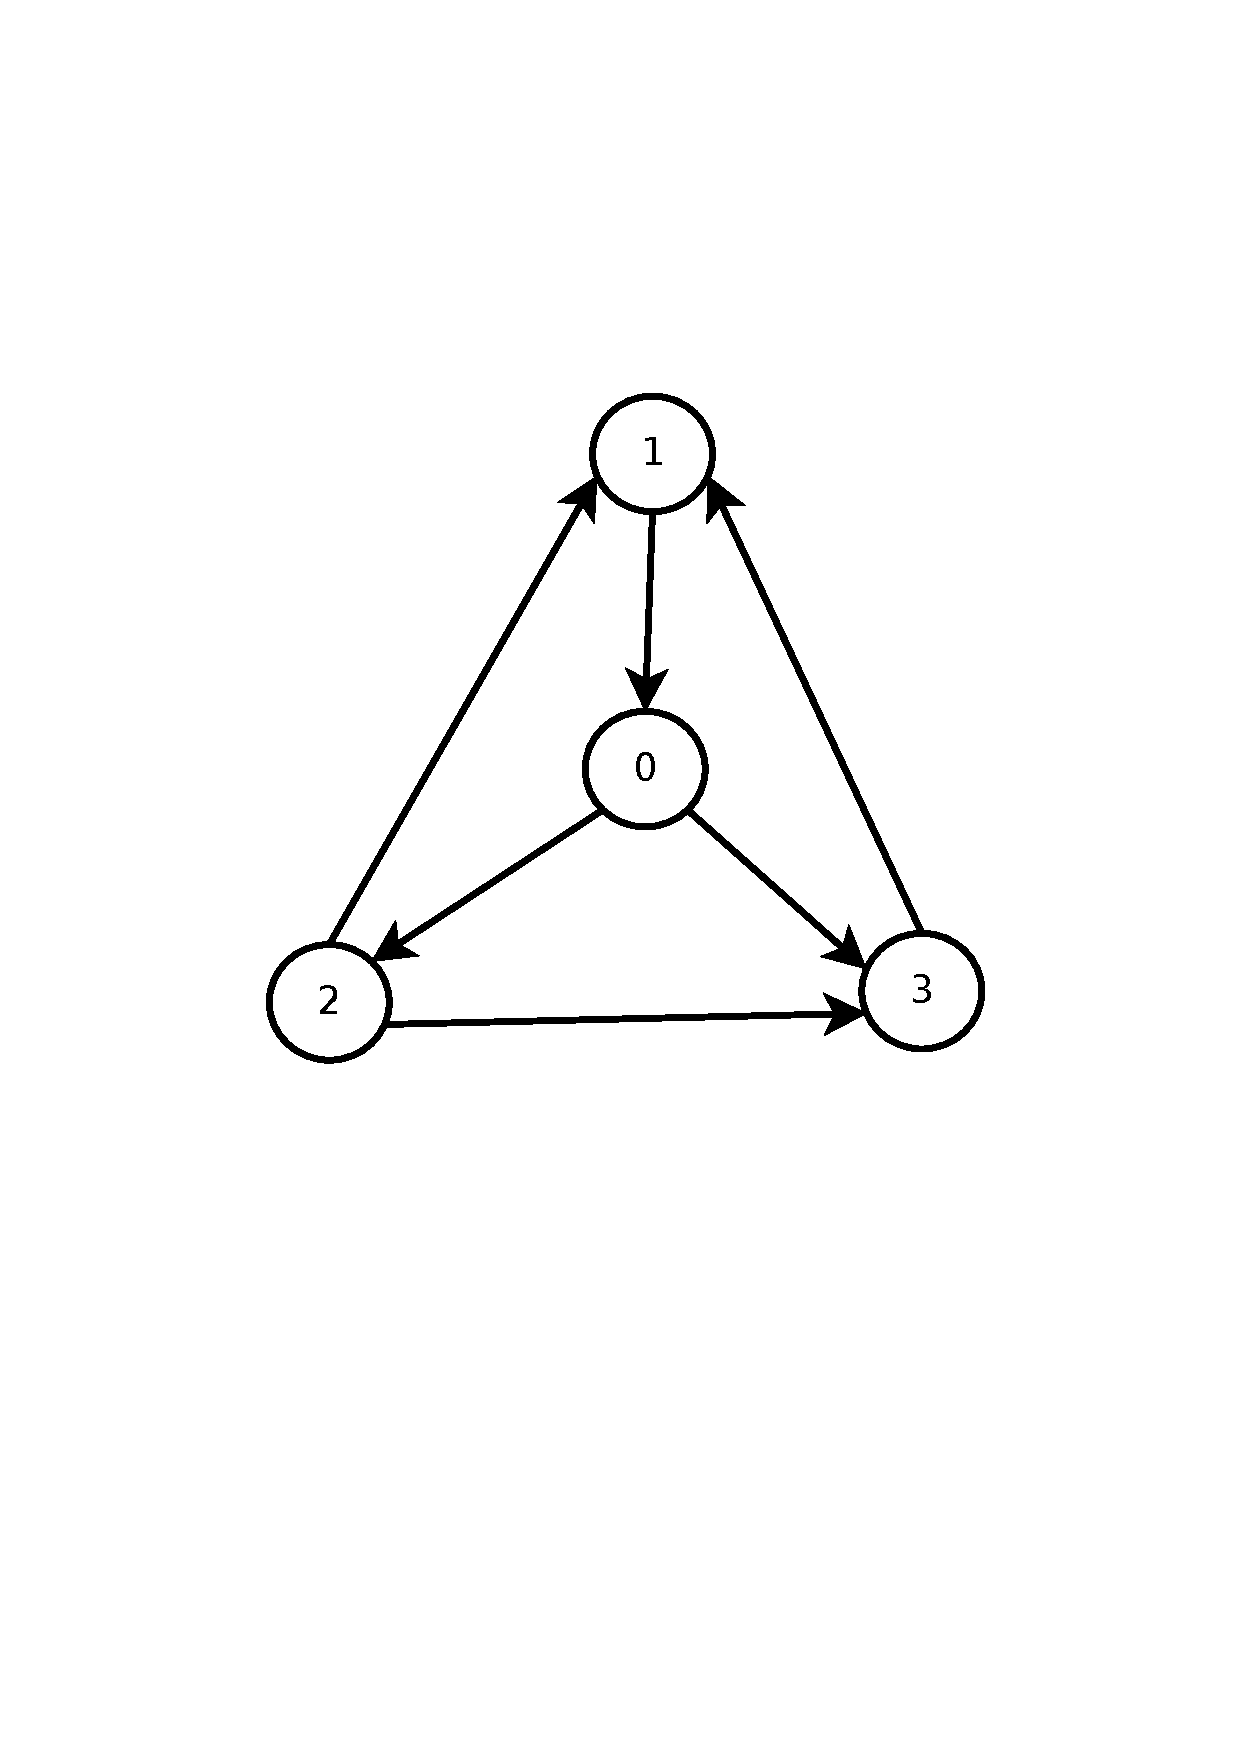
\includegraphics[scale=0.30]{exemple1_graphe.pdf}
\end{center}

Les représentatons par matrice et liste d'adjacence sont données ci-après.

\begin{center}
   \begin{tabular}{| c | c | }
     \hline
     \textbf{Matrice d'adjacence} 	& \textbf{Liste d'adjacence}\\
     \hline
$
\begin{pmatrix} 
 0 & 0 & 1 & 1 \\
 1 & 0 & 0 & 0 \\
 0 & 1 & 0 & 1 \\
 0 & 1 & 0 & 0 \\
 \end{pmatrix}
$
& 
	\begin{tabular}{|l|l|}
  	\hline
  	$0$ & $\{2, 3\}$ \\\hline
  	$1$ & $\{0\}$ \\\hline
  	$2$ & $\{1, 3\}$ \\\hline
  	$3$ & $\{1\}$ \\
  	\hline
   	\end{tabular}
   	
   \\
   \hline
   \end{tabular}
 \end{center}



%%%
\subsection{Espace mémoire}
\begin{center}
   \begin{tabular}{| l | l | }
     \hline
     \textbf{Matrice d'adjacence} 	& \textbf{Liste d'adjacence}\\
     \hline
     $O(n^2)$						& $O(n+m)$             	   \\ 
     \hline
   \end{tabular}
 \end{center}


%%%
\subsection{Complexité de quelques opérations}
\begin{center}
   \begin{tabular}{| l | l | l | }
     \hline
     \textbf{Opérations} 							& \textbf{Matrice d'adjacence} & \textbf{Liste d'adjacence} \\
     \hline
     Tester l'existence d'un arc $s\rightarrow s'$		& $O(1)$ 						& $O(|\Succ(s)|)$ \\
     \hline
     Retourner les sommets adjacents à un sommet		& $O(n)$ 						& $O(1)$ \\
     \hline
     Parcourir l'ensemble des arcs	 				& $O(n^2)$ 					& $O(m)$ \\
     \hline
   \end{tabular}
 \end{center}


\blue{
\begin{fLemma}
$$
\sum_{s\in S} |\Succ(s)| =  |A|
$$
\end{fLemma}
} 
 
%%%
\subsection{Choix d'utilisation}
\begin{itemize}
	\item D'une manière générale, on considère que si le graphe a  "peu" d'arêtes, il
	est plus intéressant d'utiliser une représentation par liste d'adjacence, plutôt que par
	matrice d'adjacence (qui contiendrait alors beaucoup de $0$).
	\item Mais si le graphe a "beaucoup" d'arêtes, il est plus intéressant d'utiliser 
	une matrice d'adjacence.
\end{itemize}



\newpage
\section{Parcours en largeur de graphes
\\ (\textit{Breadth First Search}) }



\begin{algorithm}[H]
\caption{$\algo{BFS}( G=(S, \Succ), s_0 )$}
\begin{algorithmic}[1]
\State $done \gets $ Liste vide
\State $todo\gets $ File vide
\State $todo.\enfiler(s_0)$
\State $done.\append(s_0)$
\While{$todo$ non vide}
	\State $s\gets todo.\defiler()$
	\For{$s'\in \Succ(s)$}
		\If{$s' \notin done$}
			\State $todo.\enfiler(s')$
			\State $done.\append(s')$
		\EndIf
	\EndFor
\EndWhile
\State\Return $done$
\end{algorithmic}
\end{algorithm}



\newpage
\section{Problème de l'arrêt}


\blue{
\begin{fDefinition}[\textsc{Arrêt}]
$\\$
\noindent
\underline{Entrées :}
\begin{enumerate}
\item \textup{\texttt{<Prog>}} : le code source d'un programme \textup{\texttt{Prog}} ;
\item \textup{\texttt{x}} : une entrée pour \textup{\texttt{Prog}}.
\end{enumerate}
\underline{Sortie :} \textup{\texttt{Prog(x)}} s'arrête-t-il ?
\end{fDefinition}
}

\blue{
\begin{fTheorem}[Turing]
\textsc{Arrêt} est indécidable.
\end{fTheorem}
}
\begin{proof}[Preuve]
(Par l'absurde).
On suppose qu'\textsc{Arrêt} est décidable ; i.e.
il existe un programme, 
soit \texttt{Halt}, qui décide le problème de l'arrêt ;
i.e., pour tout programme \texttt{Prog} de code source \texttt{<Prog>}, 
pour toute entrée \texttt{x} de \texttt{Prog} : 
\begin{itemize}
\item
	\texttt{Prog(x)} s'arrête $\iff$
	\texttt{Halt(<Prog>, x)} répond \texttt{Vrai} ;
\item
	\texttt{Prog(x)} ne s'arrête pas $\iff$
	\texttt{Halt(<Prog>, x)} répond \texttt{Faux}.
\end{itemize}

On considère le programme \texttt{Diagonale} ci-après :

\begin{verbatim}
Diagonale(y):
    Si Halt(y, y) = Vrai :
        opérer une boucle infinie
    Sinon
        retourner "toto"
    Fin Si
\end{verbatim}

Nous considérons l'exécution : \texttt{Diagonale(<Diagonale>)}.
\begin{enumerate}[(a)]
\item \underline{Cas 1 : \texttt{Halt(<Diagonale>, <Diagonale>) = Vrai}}

D'après le code de \texttt{Diagonale}, il suit que 
\texttt{Diagonale(<Diagonale>)} ne s'arrête pas, donc que 
\texttt{Halt(<Diagonale>, <Diagonale>)} répond \texttt{Faux}.

\item \underline{Cas 2 : \texttt{Halt(<Diagonale>, <Diagonale>) = Faux}}

D'après le code de \texttt{Diagonale}, il suit que 
\texttt{Diagonale(<Diagonale>)} s'arrête, donc que 
\texttt{Halt(<Diagonale>, <Diagonale>)} répond \texttt{Vrai}.
\end{enumerate}
%
\end{proof}

%%%%%%%%%%%%%%%%%%%%%%%%%%%%%%%%%%%%%%%%%%%%%%%%%%%%%%%%%%%%%%%
%\Section{\textsc{Ramasse-miette}}
%\begin{definition*}[\textsc{Ramasse-miette}]
%$~$
%
%\noindent
%\underline{Entrées :}
%\begin{enumerate}
%\item \texttt{Prog} : un programme;
%\item \texttt{x} : une entrée pour \texttt{Prog}.
%\end{enumerate}
%\underline{Sortie :} \texttt{Prog(x)} s'arrête-t-il ?
%\end{definition*}
%
%\begin{theoreme*}[Turing]
%\textsc{Arrêt} est indécidable.
%\end{theoreme*}
%%
%\begin{proof}[Preuve]
%\end{proof}




\newpage
\section{Approche des problèmes d’optimisation}


Nous considérons une veille radio que l’on trouve dans une brocante ; 
elle comporte une molette : $A$ ; et 3 boutons : $B$, $C$ et $D$.

\begin{itemize}
\item	$A$ permet de capter des fréquences (100 fréquences disponibles) ; 
\item	$B$, $C$ et $D$ sont trois boutons qui peuvent prendre 10 valeurs chacune 
	-- mais dont on ne connait la signification.
\end{itemize}

Une solution est la donnée d’un quadruplet $(a, b, c, d)$ 
où $a$, $b$, $c$ et $d$ indiquent des positions, 
de la molette
et des différents boutons.

Au total : $100 \times 10 \times 10 \times 10 = 100~000$ solutions possibles.

Le but est de trouver une station diffusant une chanson que l’on aime bien, et 
avec une bonne qualité de diffusion.

Pour chaque solution, i.e. chaque possibilité de quadruplet, on donne une note.


\subsubsection*{Exemple de notation.}

On entend :
\begin{itemize}
\item	Seulement des bruits de grésillement $\rightarrow 0/20$ ;
\item	Des voix, avec beaucoup de grésillement $\rightarrow 5/20$ ;
\item	Une chanson avec grésillement $\rightarrow 12/20$ ;
\item	Des voix ; avec bonne qualité d’écoute $\rightarrow 14/20$ ;
\item	Une chanson « sympathique » ; avec bonne qualité d’écoute $\rightarrow 17/20$ ;
\item	Une chanson que l’on aime davantage ; avec bonne qualité d’écoute $\rightarrow 19/20$.
\end{itemize}

Nous nous faisons face à un problème d’\textbf{optimisation} ; 
il s’agit, en effet, de trouver une solution qui \textbf{maximise} la note.

Etant donné le nombre de solutions possibles 
 ; on utilise alors une heuristique de résolution.
(Tester 100 000 configurations possibles n’est pas acceptable pour un humain).






%-----------------------------------------
%\newpage
%\section{Résolution exacte par backtracking}
%A VENIR
%\input{14__backtracking}

\newpage
\section{Algorithmes de type glouton}



\blue{
\begin{fDefinition}[Heuristique]
Une heuristique (du grec ancien "eurisko" 
« je trouve ») est une méthode de calcul qui fournit "rapidement" une solution "réalisable" 
(non nécessairement optimale ou exacte)
 pour un problème d'optimisation "difficile".
\end{fDefinition}
}

\textbf{Note :} 
Une heuristique s'impose quand les algorithmes de résolution exacte 
sont de complexité exponentielle, et dans beaucoup de problèmes "difficiles". 
L'usage d'une heuristique est également pertinent pour calculer une solution approchée 
d'un problème, ou encore pour "accélérer" un processus de résolution exacte. 
Généralement, une heuristique est conçue pour un problème particulier, 
en s'appuyant sur sa structure propre, mais peut contenir des principes 
plus généraux.

\blue{
\begin{fDefinition}[Algorithme glouton]
Un algorithme glouton (greedy algorithm en anglais) est un algorithme qui 
suit le principe de faire, étape par étape, un choix optimum (local). 
Dans certains cas, cette approche permet d'arriver à un optimum global ; 
mais dans le cas général, c'est une heuristique.
\end{fDefinition}
}






\newpage
\section{Problème de la somme du sous-ensemble 
\\ (\textit{Subset Sum Problem})}

%%%
\subsection{Définition du problème}
%%%
%%%
\blue{
\begin{fDefinition}[Problème de la somme du sous-ensemble]
$~$
\begin{itemize} 
	\item \textup{Entrée.}
		\begin{itemize}
			\item Un tableau $t$, de taille $n$, à valeurs entières.
			\item Une capacité $c\in \mathbb{N}$.
		\end{itemize}
	\item \textup{Problème.}
		\begin{itemize}
			\item[]Trouver $k$ indices de $t$,  distincts, soient $i_1, ..., i_k$, tels que la somme : 
			$$t[i_1] + ... + t[i_k]$$
			Approche la capacité $c$, sans la dépasser.
		\end{itemize}
\end{itemize}
\end{fDefinition}
}

\blue{
\begin{fTheorem}
Le problème de la somme du sous-ensemble
est NP-hard. 
\end{fTheorem}
}

\begin{proof}
Admis.
\end{proof}
%%%
%%%
%%%
%%%
%%%
%%%
\subsection{Heuristique gloutonne}
%%%
%%%

\begin{algorithm}[H]
\caption{$\algo{greedy}(t, n, c)$}
\begin{algorithmic}[1]
\State trier $t$ selon l'ordre décroissant
\State $res \gets $ Liste vide
\State $val \gets 0$
\For{$i \gets 0, ..., n-1$}
	\If{$val + t[i] \leq c$}
		\State $res.\append(i)$	
		\State $val \gets val + t[i]$
	\EndIf
\EndFor
\State\Return $res$
\end{algorithmic}
\end{algorithm}

Complexité : $O(n . \log n)$.



%-----------------------------------------
\newpage
\section{Problème de la coloration de graphe 
\\ (\textit{Graph Coloring Problem})}


\subsection{Définition du problème}
%%%
%%%
\blue{
\begin{fDefinition}[Problème de la coloration de graphe]
$~$
\begin{itemize} 
	\item \textup{Entrée.}
		\begin{itemize}
			\item[] Un graphe $G$, non orienté sans boucle.
		\end{itemize}
	\item \textup{Problème.}
		\begin{itemize}
			\item[] Trouver le plus petit entier $k$, tel que $G$ soit $k$-colorable.
		\end{itemize}
\end{itemize}
\end{fDefinition}
}

\blue{
\begin{fTheorem}
Le problème de la coloration de graphe est NP-hard. 
\end{fTheorem}
}

\begin{proof}
Admis.
\end{proof}
%%%
%%%
%%%
%%%
%%%
%%%
\subsection{Coloration gloutonne}
%%%
%%%

\begin{algorithm}[H]
\caption{$\algo{Greedy\_Colouring}( G=(S, A) )$ 
	tel que $S=\{s_{i} : i\in\{0, ..., n-1\} \}$}
\begin{algorithmic}[1]
\State $color \gets$ un dictionnaire vérifiant : $\forall s\in S, color[s]=-1$
\For{$i\gets 0, .., n-1$}
	\State $C_i \gets \{color[s_j] : (s_i, s_j)\in A\}$ 
	\State $color[s_i] \gets \min \{c\in\mathbb{N} : c\notin C_i \}$
		\green{\Comment{Le plus petit entier positif n'appartenant pas à $C_i$}}
\EndFor
\State\Return $color$
\end{algorithmic}
\end{algorithm}

%Complexité : $O(n^2)$

% \blue{
% \begin{fTheorem}
% L'algorithme $\textsc{Greedy\_Colouring}$ donne une coloration de graphe.
% \end{fTheorem}
% }

% \blue{
% \begin{fLemma} Après déroulement de $\textsc{Greedy\_Colouring}$, tout sommet est coloré.
% \end{fLemma}
% }

% Autrement dit : $\forall s\in S, color[s]>-1$.

% \begin{proof}
% L'algorithme assure, que le dictionnaire retourné $color$, vérifie :
% $$\forall s\in S, color[s]\in \mathbb{N}$$
% \end{proof}


% \blue{
% \begin{fLemma}
% $\forall i\not=j, color[s_i]\not= color[s_j]$
% \end{fLemma}
% }

% \begin{proof}
% Par l'absurde, supposons $i$ et $j$ tels que $color[v_i]=color[v_j]$.
% Sans perte de généralité, supposons $i>j$. Contradiction d'après la proposition 1.
% \end{proof}





\newpage
\section{Problème du voyageur de commerce 
\\(\textit{Travelling Salesman Problem})}

%%%
\subsection{Définition du problème}
%%%
%%%
\blue{
\begin{fDefinition}[Cycle hamiltonien]
Un cycle hamiltonien (d'un graphe)
est un cycle passant par tous les sommets du graphe, une fois et une seule.
\end{fDefinition}
}

\blue{
\begin{fDefinition}[Problème du voyageur de commerce]
$~$
\begin{itemize} 
	\item \textup{Entrée.}
		\begin{itemize}
			\item[] Un graphe $G=(S, A, cost)$, tel que : 
			\begin{itemize}
				\item[--] $G$ est non orienté ; 
				\item[--] $G$ est complet ;
				\item[--] Les arcs de $G$ sont valués par la fonction $cost : A\rightarrow \mathbb{R}$.
			\end{itemize}
		\end{itemize}
	\item \textup{Problème.}
		\begin{itemize}
			\item[] Trouver le cycle hamiltonien ayant le coût le plus faible.
		\end{itemize}
\end{itemize}
\end{fDefinition}
}

\blue{
\begin{fTheorem}
Le problème du voyageur de commerce est NP-hard. 
\end{fTheorem}
}

\begin{proof}
Admis.
\end{proof}
%%%
%%%
%%%
%%%
%%%
%%%
\subsection{Heuristique : algorithme du plus proche voisin}
%%%
%%%

\begin{algorithm}[H]
\caption{$\algo{nearest\_neighbour}( G=(S, A, cost) )$}
\begin{algorithmic}[1]
\State $todo \gets \{\}$
\State $res \gets $ Liste vide
\State $s_0 \gets $ choisir un sommet arbitraire de $G$
\State $todo\gets G-\{s_0\}$
\State $res.\append(s_0)$
\State $s\gets s_0$
\While{$todo\not=\{\}$}
	\State $s' \gets$ le sommet le plus proche de $s$
	\State $todo\gets todo - \{s'\}$
	\State $res.\append(s')$
	\State $s\gets s'$
\EndWhile
\State\Return $res.\append(s_0)$
\end{algorithmic}
\end{algorithm}

%Complexité : $O(n^2)$ ???



\newpage
\section{Algorithmes génétiques}


On cherche à maximiser $f : E \rightarrow \mathbb{R}$ ; où  $E$  est fini.

Exemple (pour un entier $n$) :  
\begin{itemize}
	\item $E=\texttt{float}^n$ ;
	\item $E=\mathbb{B}^n$ ;
	\item $E=\{x_1, ..., x_k\}^n$  (pour un entier $k$) ;
	\item $E=S_n$ (l'ensemble des permutations de \{1, ..., n\}).
\end{itemize}


\begin{algorithm}[H]
\caption{\algo{algorithme\_genetique}(
	$n$ : taille d'un individu, 
	$\newline$
	$~~~~~~~~~~~~~~~~~~~~~~~~~~~~~~~~~~~~~~~~~~~~~~~~~~~~~~~~~$ 
	$p$ : nombre d'individus, ...)}
\begin{algorithmic}[1]
\State $P \gets$ Population initiale
\State 	$res \gets \Null$
			\green{\Comment{En considérant $f(\Null) = - \infty$}}
\While{$\Not$(Critère Fin)}
	\State Calculer la valeur de fitness de chaque individu   
			\green{\Comment{i.e. $f(p), \forall p\in P$}}
	\State $best \gets $ le meilleur individu de $P$ 
			\green{\Comment{Au sens de la maximisation de $f$}}
  	\If{ $f(best) > f(res)$}
		\State $res \gets best$
	\EndIf
	\State $P \gets selection(P)$
	\State $P_{new} \gets reproduction(P)$
	\State $P_{new} \gets mutation(P_{new})$
	\State $P \gets P_{new}$
\EndWhile
\State\Return $res$
\end{algorithmic}
\end{algorithm}

(Les phases de $selection$ et de $reproduction$
peuvent être regroupées en une procédure).


\end{document}